\documentclass{beamer}
\usepackage[utf8]{inputenc}
\usepackage[T1]{fontenc}
\usepackage{graphicx}
\usepackage{xcolor}
\usepackage{listings}
\usepackage{tikz}
\usepackage{amsmath}
\usepackage{hyperref}

% Theme - Import oppstar theme from beamer-template directory
% Add beamer-template directory to LaTeX search path
\makeatletter
\def\input@path{{./beamer-template/}}
\makeatother

% Now load the theme components
\usepackage{./beamer-template/beamercolorthemeoppstar}
\usepackage{./beamer-template/beamerfontthemeoppstar}
\usepackage{./beamer-template/beamerinnerthemeoppstar}
\usepackage{./beamer-template/beamerouterthemeoppstar}
\usepackage{./beamer-template/beamerthemeoppstar}

% Colors
\definecolor{codeblue}{RGB}{0,102,204}
\definecolor{codegray}{RGB}{128,128,128}
\definecolor{codegreen}{RGB}{0,128,0}
\definecolor{backcolour}{RGB}{245,245,245}

% Code listing style
\lstdefinestyle{cstyle}{
    backgroundcolor=\color{backcolour},
    commentstyle=\color{codegreen},
    keywordstyle=\color{codeblue},
    numberstyle=\tiny\color{codegray},
    stringstyle=\color{red},
    basicstyle=\ttfamily\tiny,
    breakatwhitespace=false,
    breaklines=true,
    keepspaces=true,
    numbers=left,
    numbersep=5pt,
    showspaces=false,
    showstringspaces=false,
    showtabs=false,
    tabsize=2,
    frame=single
}

\lstset{style=cstyle}

% Title page info
\title{Day 2: Control Flow and Debugging}
\subtitle{C Programming for Post-Silicon Validation Engineers}
\author{Yahwista Salomo}
\date{6-Day Intensive Bootcamp}
\institute{Post-Silicon Validation Training Program}

\begin{document}

\frame{\titlepage}

\begin{frame}
\frametitle{Welcome to Day 2!}
\begin{center}
\Large Making Decisions and Finding Bugs
\end{center}

\begin{itemize}
    \item \textbf{Yesterday:} Basic C syntax and compilation
    \item \textbf{Today's Mission:} Control flow and debugging mastery
    \item \textbf{Validation Focus:} Test sequences and fault detection
    \item \textbf{New Tool:} GDB debugger
    \item \textbf{Outcome:} Automated register monitoring system!
\end{itemize}

\vspace{0.5cm}
\begin{center}
\textit{"Programs must be written for people to read, and only incidentally for machines to execute"} - Abelson \& Sussman
\end{center}
\end{frame}

\begin{frame}
\frametitle{Today's Learning Objectives}
By the end of Day 2, you will:

\begin{enumerate}
    \item Master conditional statements (if-else)
    \item Implement loops for repetitive testing
    \item Create and call functions effectively
    \item Use GDB to debug programs step-by-step
    \item Design automated test sequences
    \item Handle multiple validation scenarios
\end{enumerate}

\vspace{0.5cm}
\begin{alertblock}{Validation Context}
Build test sequences that simulate real hardware monitoring!
\end{alertblock}
\end{frame}

\begin{frame}[fragile]
\frametitle{Conditional Statements - Making Decisions}
\begin{lstlisting}[language=C]
#include <stdio.h>

int main() {
    float temperature = 75.5;
    float max_temp = 85.0;

    if (temperature > max_temp) {
        printf("CRITICAL: Temperature too high!\\n");
        printf("Shutting down for safety...\\n");
    } else if (temperature > max_temp - 10) {
        printf("WARNING: Temperature approaching limit\\n");
    } else {
        printf("Temperature normal: %.1f\\textdegree C\\n", temperature);
    }

    return 0;
}
\end{lstlisting}

\textbf{Key points:}
\begin{itemize}
    \item Use \texttt{==} for equality, not \texttt{=}
    \item Combine conditions with \texttt{\&\&} (AND) and \texttt{||} (OR)
    \item Always use braces \texttt{\{\}} for clarity
\end{itemize}
\end{frame}

\begin{frame}
\frametitle{Logical Operators in Validation}
\begin{center}
\begin{tabular}{|l|l|l|}
\hline
\textbf{Operator} & \textbf{Meaning} & \textbf{Validation Example} \\
\hline
\texttt{\&\&} & AND & \texttt{voltage > 1.8 \&\& voltage < 3.6} \\
\texttt{||} & OR & \texttt{error\_code == 1 || error\_code == 2} \\
\texttt{!} & NOT & \texttt{!system\_ready} \\
\hline
\end{tabular}
\end{center}

\vspace{0.5cm}
\begin{exampleblock}{Complex Validation Logic}
\texttt{if (voltage >= min\_v \&\& voltage <= max\_v \&\& !error\_flag) \{\\
\quad // System is ready for testing\\
\}}
\end{exampleblock}

\vspace{0.5cm}
\textbf{Validation Tip:} Always check multiple parameters for robust testing!
\end{frame}

\begin{frame}[fragile]
\frametitle{Loops - Repetitive Testing}
\textbf{For Loop - Known iterations:}
\begin{lstlisting}[language=C]
// Test 8 consecutive registers
for (int i = 0; i < 8; i++) {
    int reg_addr = 0x1000 + i;
    int value = read_register(reg_addr);
    printf("Register 0x%04X: 0x%04X\\n", reg_addr, value);
}
\end{lstlisting}

\textbf{While Loop - Condition-based:}
\begin{lstlisting}[language=C]
// Keep testing until system is ready
while (!system_ready()) {
    printf("Waiting for system initialization...\\n");
    sleep(1);  // Wait 1 second
}
printf("System ready for validation!\\n");
\end{lstlisting}
\end{frame}

\begin{frame}[fragile]
\frametitle{Functions - Modular Testing}
\begin{lstlisting}[language=C]
#include <stdio.h>

// Function to validate voltage range
int check_voltage(float voltage, float min, float max) {
    if (voltage < min || voltage > max) {
        printf("FAIL: Voltage %.2fV out of range [%.1f-%.1f]\\n",
               voltage, min, max);
        return 0;  // Fail
    }
    printf("PASS: Voltage %.2fV within range\\n", voltage);
    return 1;  // Pass
}

int main() {
    float test_voltage = 3.3;
    int result = check_voltage(test_voltage, 1.8, 3.6);

    if (result) {
        printf("Voltage test passed!\\n");
    } else {
        printf("Voltage test failed!\\n");
    }
    return 0;
}
\end{lstlisting}
\end{frame}

\begin{frame}
\frametitle{Function Anatomy}
\begin{center}
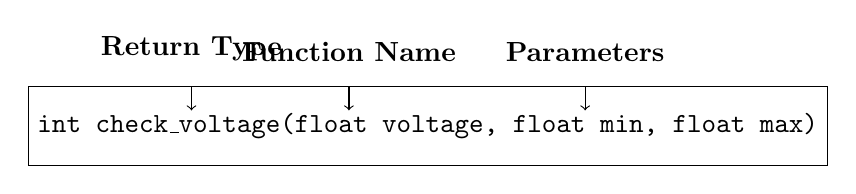
\begin{tikzpicture}
\node[draw, rectangle, minimum width=8cm, minimum height=1cm] at (0,0)
{\texttt{int check\_voltage(float voltage, float min, float max)}};

\node[above] at (-3,0.7) {\textbf{Return Type}};
\draw[->] (-3,0.5) -- (-3,0.2);

\node[above] at (-1,0.7) {\textbf{Function Name}};
\draw[->] (-1,0.5) -- (-1,0.2);

\node[above] at (2,0.7) {\textbf{Parameters}};
\draw[->] (2,0.5) -- (2,0.2);
\end{tikzpicture}
\end{center}

\textbf{Function Benefits:}
\begin{itemize}
    \item \textbf{Reusability:} Write once, use many times
    \item \textbf{Modularity:} Break complex problems into smaller pieces
    \item \textbf{Testing:} Easier to test individual components
    \item \textbf{Maintenance:} Changes in one place affect everywhere
\end{itemize}

\vspace{0.5cm}
\textbf{Validation Tip:} Create separate functions for each test type!
\end{frame}

\begin{frame}[fragile]
\frametitle{Introduction to GDB - Your Debugging Friend}
\textbf{Compile with debug symbols:}
\begin{verbatim}
$ gcc -g -Wall program.c -o program
\end{verbatim}

\textbf{Start GDB:}
\begin{verbatim}
$ gdb ./program
(gdb) break main          # Set breakpoint at main
(gdb) run                 # Start program
(gdb) next                # Execute next line
(gdb) print voltage       # Show variable value
(gdb) continue            # Continue execution
(gdb) quit                # Exit GDB
\end{verbatim}

\textbf{Why GDB for validation?}
\begin{itemize}
    \item Step through test sequences
    \item Inspect register values
    \item Find where tests fail
    \item Understand program flow
\end{itemize}
\end{frame}

\begin{frame}[fragile]
\frametitle{GDB Commands for Validation}
\begin{center}
\begin{tabular}{|l|l|}
\hline
\textbf{Command} & \textbf{Purpose} \\
\hline
\texttt{break function\_name} & Set breakpoint \\
\texttt{run} & Start program \\
\texttt{next} & Execute next line \\
\texttt{step} & Step into functions \\
\texttt{print variable} & Show variable value \\
\texttt{info locals} & Show all local variables \\
\texttt{backtrace} & Show call stack \\
\texttt{continue} & Resume execution \\
\hline
\end{tabular}
\end{center}

\vspace{0.5cm}
\begin{exampleblock}{Debugging Session}
\texttt{(gdb) break check\_voltage}\\
\texttt{(gdb) run}\\
\texttt{(gdb) print voltage}\\
\texttt{(gdb) next}
\end{exampleblock}
\end{frame}

\begin{frame}[fragile]
\frametitle{Validation Example: Register Monitor}
\begin{lstlisting}[language=C, basicstyle=\tiny]
#include <stdio.h>

// Simulate reading hardware register
int read_register(int address) {
    // In real hardware: return *(volatile int*)address;
    static int sim_values[] = {0x1234, 0x5678, 0x9ABC, 0xDEF0};
    return sim_values[address % 4];
}

// Validate single register
int validate_register(int address, int expected) {
    int actual = read_register(address);
    printf("Reg 0x%04X: Expected=0x%04X, Actual=0x%04X ",
           address, expected, actual);

    if (actual == expected) {
        printf("PASS\\n");
        return 1;
    } else {
        printf("FAIL\\n");
        return 0;
    }
}

// Run complete register test suite
int run_register_tests() {
    int passed = 0;
    int total = 4;

    passed += validate_register(0x1000, 0x1234);
    passed += validate_register(0x1001, 0x5678);
    passed += validate_register(0x1002, 0x9ABC);
    passed += validate_register(0x1003, 0xDEF0);

    printf("\nResults: %d/%d tests passed\\n", passed, total);
    return (passed == total);
}
\end{lstlisting}
\end{frame}

\begin{frame}[fragile]
\frametitle{Advanced Control: Switch Statements}
\begin{lstlisting}[language=C]
void handle_error_code(int error) {
    switch (error) {
        case 0:
            printf("No error - system OK\\n");
            break;
        case 1:
            printf("Voltage out of range\\n");
            break;
        case 2:
            printf("Temperature too high\\n");
            break;
        case 3:
            printf("Clock not locked\\n");
            break;
        default:
            printf("Unknown error code: %d\\n", error);
            break;
    }
}
\end{lstlisting}

\textbf{When to use switch:}
\begin{itemize}
    \item Multiple discrete values to check
    \item Error code handling
    \item State machine implementation
\end{itemize}
\end{frame}

\begin{frame}[fragile]
\frametitle{Interactive Poll: Debug This!}
\begin{center}
\Large What's wrong with this code?
\end{center}

\begin{lstlisting}[language=C]
int voltage = 3.3;
if (voltage = 3.3) {
    printf("Voltage is correct\\n");
}
\end{lstlisting}

\pause

\begin{alertblock}{Answer}
Using assignment \texttt{=} instead of comparison \texttt{==}!\\
Should be: \texttt{if (voltage == 3.3)}
\end{alertblock}

\vspace{0.5cm}
\textbf{Pro tip:} GCC with \texttt{-Wall} would warn about this!
\end{frame}

\begin{frame}[fragile]
\frametitle{Common Debugging Scenarios}
\textbf{Infinite Loop:}
\begin{lstlisting}[language=C]
// BUG: Counter never increments
int i = 0;
while (i < 10) {
    printf("Testing register %d\\n", i);
    // Missing: i++;
}
\end{lstlisting}

\textbf{Off-by-One Error:}
\begin{lstlisting}[language=C]
// BUG: Should be i < 8, not i <= 8
for (int i = 0; i <= 8; i++) {
    test_register(base_addr + i);  // Accesses 9 registers!
}
\end{lstlisting}

\textbf{Uninitialized Variable:}
\begin{lstlisting}[language=C]
int error_count;  // BUG: Not initialized
error_count += check_voltage();  // Undefined behavior!
\end{lstlisting}
\end{frame}

\begin{frame}
\frametitle{Validation Test Design Patterns}
\textbf{1. Sequential Testing:}
\begin{itemize}
    \item Test registers in order
    \item Stop on first failure vs. continue testing
    \item Log all results for analysis
\end{itemize}

\textbf{2. Boundary Testing:}
\begin{itemize}
    \item Test minimum and maximum values
    \item Test just inside and outside valid ranges
    \item Critical for voltage and timing validation
\end{itemize}

\textbf{3. Stress Testing:}
\begin{itemize}
    \item Repeat tests many times
    \item Look for intermittent failures
    \item Essential for reliability validation
\end{itemize}

\vspace{0.5cm}
\begin{center}
\textbf{Good test design finds bugs before customers do!}
\end{center}
\end{frame}

\begin{frame}
\frametitle{Lab Preview: Register Monitoring System}
\textbf{This afternoon you'll build:}
\begin{itemize}
    \item Multi-register validation suite
    \item Configurable test parameters
    \item Detailed pass/fail reporting
    \item Error logging and analysis
    \item GDB debugging session documentation
\end{itemize}

\vspace{0.5cm}
\textbf{Features to implement:}
\begin{itemize}
    \item Loop through register ranges
    \item Function-based test organization
    \item Conditional error handling
    \item Summary statistics
    \item Debug with GDB and document findings
\end{itemize}
\end{frame}

\begin{frame}
\frametitle{Key Takeaways - Day 2}
\begin{itemize}
    \item \textbf{Control flow is power:} Make your programs smart and adaptive
    \item \textbf{Functions are essential:} Modular code is maintainable code
    \item \textbf{Loops enable automation:} Test hundreds of registers effortlessly
    \item \textbf{GDB is your ally:} Debug systematically, not by guessing
    \item \textbf{Design for validation:} Think about edge cases and error conditions
\end{itemize}

\vspace{0.5cm}
\begin{center}
\textbf{You're building real validation tools now!}
\end{center}
\end{frame}

\begin{frame}
\frametitle{Tonight's Homework}
\textbf{Enhance your register monitor:}
\begin{enumerate}
    \item Add nested loops for multi-chip testing
    \item Implement error recovery mechanisms
    \item Create summary statistics functions
    \item Use GDB to trace through your program
    \item Document debugging findings in README
\end{enumerate}

\vspace{0.5cm}
\textbf{Debugging challenge:}
\begin{itemize}
    \item Intentionally introduce a bug
    \item Use GDB to find and fix it
    \item Document the debugging process
\end{itemize}
\end{frame}

\begin{frame}
\frametitle{Tomorrow Preview: Memory and Pointers}
\begin{center}
\Large Get ready for the most important day!
\end{center}

\textbf{Day 3 topics:}
\begin{itemize}
    \item Pointers and memory addressing
    \item Arrays for bulk data handling
    \item Structures for chip modeling
    \item Bit manipulation for register control
    \item Introduction to AI coding assistants
\end{itemize}

\vspace{0.5cm}
\begin{alertblock}{Preparation}
Review today's pointer examples and practice with GDB!
\end{alertblock}
\end{frame}

\begin{frame}
\frametitle{Questions \& Discussion}
\begin{center}
\Large Let's debug together!
\end{center}

\begin{itemize}
    \item Any control flow concepts need clarification?
    \item GDB questions or troubleshooting needs?
    \item How do these patterns apply to your validation scenarios?
    \item Ready to tackle more complex programs?
\end{itemize}

\vspace{1cm}
\begin{center}
\textbf{Time for hands-on debugging practice!}
\end{center}
\end{frame}

\end{document}

